\chapter{TAkka: Design and Implementation}
\label{takka_design}

\begin{center}
A condensed version of the material in this chapter appears \\ in~\citep[Section 3 and 4]{TAKKA_paper}
\end{center}
\vspace{12 pt}

The last chapter examined actor programming and supervision in Erlang/OTP and Akka. 
 Erlang/OTP is written in Erlang, a dynamically typed language, whereas Akka is 
written in Scala, a statically typed language. A key advantage of static typing 
is that it detects some type errors at an early stage, i.e., at compile time.  
Nevertheless, messages sent to Akka actors are dynamically typed. 

\begin{comment}
because it was believed that 
type parameterized actors and supervision will be difficult
to work together [? private communication and mailing list question ?] .
\end{comment}

This chapter presents the design of the TAkka library, which confirms the key 
claim of this thesis: actors in supervision trees can be 
{\it statically} typed by parameterizing the actor class with the type of 
messages it expects to receive.  This chapter outlines how 
static and dynamic type checking are used to prevent ill-typed messages.  
Examples of TAkka applications show that type-parameterized actors can form 
supervision trees in the same way as actors without type parameters.  This 
chapter concludes with a brief discussion on design alternatives used by 
other actor libraries.

The latest TAkka library is built on top of Akka 2.1.4.  During the research 
of this project, TAkka has been built on stable Akka releases since 2.0.  For 
all Akka versions, actors can be parameterized as expected.  
Nevertheless, as the Akka API and the structure of Akka configuration file change 
slightly in different Akka versions, readers who want to use a later Akka 
version may need to update the API or the configuration file according to the 
specification of the Akka version used.  The latest TAkka API and its companion Akka
API (version 2.1.4) are given in Appendix A.


\section{TAkka Example: a String Counter}
\label{sec:takka_example}

The introduction of TAkka begins with an illustrative TAkka example in Figure~\ref{takka_string_counter}. The example is ported from the string counter 
example given in Figure~\ref{fig:akka_string_counter}.  The TAkka code is 
similar to its Akka equivalent, with a few differences marked in 
\textcolor{blue}{blue}.  

First, the {\tt Actor} class in TAkka takes a type 
parameter which indicates the type of expected messages.  In our example, {\tt 
StringCounter} is an actor which only expects String messages.  Consequently, 
its {\tt typedReceive} function has a function type {\tt String => Unit}.  The 
type is not explicitly declared in code because it can be inferred and checked 
by the Scala type system.  In an Eclipse IDE with Scala plug-in, the following 
type information is shown on the screen when the {\tt typedReceive} 
method is mouseovered:
\begin{lstlisting}[language=scala]
  def typedReceive: String => Unit
\end{lstlisting}%
The type of {\tt m} at line 8, which is {\tt String}, is omitted too because it can be 
inferred as well.

Second, the type of messages sending to an actor reference is statically 
checked. In the TAkka version of the {\tt StringCounterTest}, the Scala 
language infers that the  type of {\tt counter}, declared at line 16, has type 
{\tt ActorRef[String]}.  This means that only String messages can be sent to {\tt 
counter}.   Sending a non-String message (i.e. line 21) results in a compile error.

Third, dynamic type checking is involved at the earliest opportunity when 
static type checking meets its limitation.  For example, when a user looks up 
an actor reference by its type and path, as at line 23 and 26, 
TAkka does not statically check if there will be an actor of a 
compatible type at that path when the program is executed.  Although the type 
error at line 26 is not statically detected, an exception is expected to raise
as soon as the ill-typed actor reference is claimed at run time (line 26), 
earlier than the time when the actor reference is used (line 29).  
The terminal output shows that the print statement
at line 28 has not been executed when the exception is raised.  The result confirms that
the exception is raised by code at line 26.



\begin{figure}
      \begin{lstlisting}[language=scala, escapechar=?]
package sample.takka

import ?\textcolor{blue}{takka}?.actor.{Actor, ActorRef, ActorSystem, Props}

class StringCounter extends ?\textcolor{blue}{Actor[String]}? {
  var counter = 0;
  def ?\textcolor{blue}{typedReceive}? = {
    case m => 
      counter = counter +1
      println("received "+counter+" message(s):\n"+m)
  }
}

object StringCounterTest extends App {
  val system = ActorSystem("StringCounterTest")
  val counter = system.actorOf(Props[?\textcolor{blue}{String}?, StringCounter], 
"counter")
  
  counter ! "Hello World"
//  counter ! 1
// type mismatch; found : Int(1) required: String  
  val counterString = 
system.actorFor?\textcolor{blue}{[String]}
?("akka://StringCounterTest/user/counter")
  counterString ! "Hello World Again"
  val counterInt = 
system.actorFor?\textcolor{blue}{[Int]}
?("akka://StringCounterTest/user/counter")  
// dynamic type error!  
  println("Hello")  // will not be executed
  counterInt ! 2      // will not be executed
}

/*
Terminal Output:

received 1 message(s):
	Hello World
received 2 message(s):
	Hello World Again
Exception in thread "main" java.lang.Exception: 
ActorRef[akka://StringCounterTest/user/counter] does not exist
or does not have type ActorRef[Int]
 */	
    \end{lstlisting}
    \caption{TAkka Example: A String Counter}
    \label{takka_string_counter}
\end{figure}


Because sending an actor a message of unexpected type is prevented,
there is no need to define a handler for unexpected messages in our TAkka
example.  Eliminating ill-typed messages benefits both users and developers
of actor-based services. For users, since messages are transmitted 
asynchronously, it is easier to trace the source of potential errors if they are 
captured earlier, especially in a distributed environment. For service 
developers, they can focus on the logic of the services rather than worrying 
about incoming messages of unexpected types.


\section{Type-parameterized Actor}
\label{takka_actor}
A TAkka actor has type {\tt Actor[M]}.  It inherits the Akka {\tt Actor} 
trait to minimize implementation effort.  Users of the TAkka library, 
however, do not need to use any Akka Actor API.  Instead, programmers are 
encouraged to use the typed interface given in Figure~\ref{takka_actor_api}.  
Unlike other actor libraries, every TAkka actor class takes a type parameter 
{\tt M} which specifies the type of messages expected by the actor.  The same 
type parameter is used as the input type of the {\tt typedReceive} function.  
The actor reference pointing to itself, {\tt typedSelf}, has type {\tt 
ActorRef[M]} to which only messages of type {\tt M} can be sent.  
The type constructor {\tt Actor} is {\it invariant} because the same type parameter is
used for {\tt ActorContext}, which is {\it invariant} as will be explained in Section~\ref{takka_actor_context}.
Finally, the actor context for the actor, {\tt typedContext}, has type {\tt ActorContext[M]}.  
%As explained 

To maintain the actor behaviour and the supervision relationship, a special class
of messages, which has type {\tt SystemMessage}, should be handled by all actors.
Unlike the Akka design, which handles system messages in the {\tt receive} block,
system messages are handled in a separate method, namely the {\tt systemMessageHandler} method.
System messages and its handler will be discussed in detail at Section~\ref{systemmessage}.


\begin{figure}[h]
\begin{lstlisting}[language=scala, escapechar=?]
package takka.actor

abstract class ?\textcolor{blue}{Actor[M:Manifest]}? extends akka.actor.Actor
  protected def ?\textcolor{blue}{typedReceive}?:?\textcolor{blue}{Function}?[?\textcolor{blue}{M}?, Unit]
  
  val ?\textcolor{blue}{typedSelf}?:ActorRef?\textcolor{blue}{[M]}?
  val ?\textcolor{blue}{typedContext}?:ActorContext?\textcolor{blue}{[M]}?
  var supervisorStrategy: SupervisorStrategy
  ?\textcolor{blue}{def systemMessageHandler:SystemMessage => Unit}?
  
  def preStart(): Unit
  def preRestart(reason: Throwable, message: Option[Any]): Unit
  def postRestart(reason: Throwable): Unit
  def postStop(): Unit
\end{lstlisting}
\caption{TAkka API: Actor}
\label{takka_actor_api}
\end{figure}

Notice that the type of {\tt typedReceive} is {\tt Function[M, Unit]}, whereas 
the type of {\tt receive} in the Akka {\tt Actor} class is {\tt 
PartialFunction[Any, Unit]}.  An 
advantage of using {\tt Function} is that the compiler can check the 
completeness of the domain patterns.  In Akka, completeness checking is not considered
because an Akka actor may receive messages of any type.  In contrast, a TAkka 
actor only expects messages of a certain type.  Therefore, pattern completeness 
checking is a helpful feature for TAkka users.

The two immutable fields of {\tt Actor}, {\tt typedContext} and 
{\tt typedSelf}, are automatically initialized when the actor is created.
Library users may override the default supervisor strategy in the
way explained in Section~\ref{supervision}.  The implementation of the {\tt
typedReceive} method, on the other hand, is always provided by users.

Types of variables and methods that do not related to message passing are not
type parameterized (i.e. {\tt supervisorStrategy}, {\tt preStart}, {\tt postRestart}, and {\tt postStop}).
The {\tt preRestart} method has the same type as the Akka version.  It is invoked before the
actor is restarted due to an error (i.e. {\tt reason}) that {\it might be} caused when processing a message (i.e. {\tt message}).
Because an actor can be evolve to a version that handles more types of messages (Section~\ref{hot_swapping}),
the type of the problematic message cannot be determined in advance.  It is fine to
define some message patterns that will never be triggered at run-time.


Notice that {\tt takka.actor.Actor} inherits {\tt akka.actor.Actor}.  A 
critical problem of using inheritance is that dynamically typed 
Akka API, which we are trying to avoid whenever possible, are still available 
to TAkka users.  Unfortunately, this limitation cannot be overcome by using 
delegation because, as we have seen in the Akka API, a child actor is created by 
calling the {\tt actorOf} method from its supervisor's actor context, which 
cannot be accessed outside the supervisor. {\tt Actor} is the only TAkka 
class that is implemented using inheritance. All other TAkka classes and traits 
are either implemented by delegating tasks to Akka counterparts or rewritten in 
TAkka.  To overcome the limitation, a complete reimplementation of that TAkka
Actor library is required.  The author estimates that the required work is
similar to implementing the Akka Actor library.


\section{Type-parameterized Actor Reference}
\label{takka_actor_ref}

The last section explains the type-parameterised Actor class, {\tt  
Actor[M]}, whose message handler only considers messages of the expected 
type {\tt M}.  Such a design only works in a system which either provides a 
reasonable handler for undefined messages at the receiver side,  or is able to 
prevent ill-typed messages at the sender side.  As mentioned in Section 
\ref{message mailbox}, undefined messages are handled differently in Erlang and 
different Akka versions.  Each mechanism has its own rationale.  
Unfortunately, there is no known single mechanism that meets the requirements of 
all applications.  The Akka development team tends to provide more ways to 
handle unexpected messages at the receiver side.  In contrast,  the TAkka 
library is aimed at preventing ill-typed messages at the sender side.  
We achieve this goal by adding a type parameter to the {\tt ActorRef} class.

The API of {\tt ActorRef} is given in Figure~\ref{takka_actor_reference_api}.  
The {\tt ActorRef} class takes two parameters: one type 
parameter that indicates the type of expected message and one implicit 
argument that records the {\tt Manifest} of the type parameter.  In most 
cases, the implicit {\tt Manifest} can be provided by the Scala language 
automatically.


\begin{figure}[h]
\begin{lstlisting}[language=scala,  escapechar=?]
package takka.actor 

abstract class ActorRef?{\textcolor{blue}{[-M](implicit mt:Manifest[M])}?
  ?{\textcolor{blue}{val untypedRef:akka.actor.ActorRef}? 

  def !(message: ?{\textcolor{blue}{M}?):Unit
  ?{\textcolor{blue}{def publishAs[SubM<:M](implicit smt:Manifest[SubM]):ActorRef[SubM]}?

  abstract def path: akka.actor.ActorPath
  final def compareTo(other: ActorRef?{\textcolor{blue}{[\_]}?): Int
  final def equals(that: Any): Boolean
  // no forward method

\end{lstlisting}
\caption{TAkka API: Actor Reference}
\label{takka_actor_reference_api}
\end{figure}

As in Erlang and Akka, users send a message to an actor via the {\tt !} 
method of its actor reference.   Sending an actor a message of a different type 
causes an error at compile time.  By using type-parameterized actor references, 
the receiver does not need to worry about unexpected messages, while senders 
can be sure that messages will be understood and processed, as long as the 
message is delivered.







\begin{figure}[p]
\begin{lstlisting}[language=scala,  escapechar=?]
package sample.takka

import takka.actor.ActorRef
import takka.actor.ActorSystem
import takka.actor.Props
import takka.actor.Actor

sealed trait Operation
case class Multiplication(m:Int, n:Int) extends Operation
case class Division(m:Int, n:Int) extends Operation

class Calculator extends Actor?{\textcolor{blue}{[Operation]}? {
  def ?{\textcolor{blue}{typedReceive}? = {
    case Multiplication(m:Int, n:Int) =>
      println(m +" * "+ n +" = "+ (m*n))    
    case Division(m, n) =>
      println(m +" / "+ n +" = "+ (m/n))
  }
}

object TAkkaActorRefTest extends App{
  val system = ActorSystem("MySystem")
  val calculator:ActorRef[Operation] = system.actorOf(Props[?{\textcolor{blue}{Operation}?, Calculator], "calculator")
  
  // explicit type conversion 
  ?{\textcolor{blue}{val multiple = calculator.publishAs[Multiplication]}?

  // implicit type conversion 
  val divide:ActorRef[Division] = calculator  
  
  calculator ! Multiplication(3, 2)
  multiple ! Multiplication(3, 3)
  //  multiple ! Division(6, 2)  
  //Compiler Error: type mismatch; found : sample.takka.Division
  //	  required: sample.takka.Multiplication
  divide ! Division(6, 2)  
}

/*
Terminal Output:
3 * 2 = 6
3 * 3 = 9
6 / 2 = 3
*/
\end{lstlisting}
\caption{TAkka Example: Typed Actor Reference}
\label{takka_actor_reference_example}
\end{figure}


An actor can usually react to a finite set of different message patterns, 
whereas our notation of actor reference only takes one type parameter.  In a 
type system that supports untagged union types, no special extension is
required.  In a type system which supports polymorphism, {\tt ActorRef} should
be contravariant on its type argument {\tt M}, denoted as {\tt ActorRef[-M]} in 
Scala.  To understand why {\tt ActorRef} is contravariant, let us consider both the 
{\it Get and Put Principle} and an illustrative example.   {\tt ActorRef} is 
contravariant because users only {\tt put} values to an actor reference (using the {\tt !} method) but 
never get values out of it.  Fetching the value sent via an actor reference is done
in the {\tt typedReceive} method of the {\tt Actor} class.  The illustrative example considered here is a 
simple calculator defined in Figure~\ref{takka_actor_reference_example}.
The calculator defined in the example can compute the result of two types of 
operations: multiplication and division.  Hence, {\tt Division} is a 
subtype of {\tt Operation}. It is clear that {\tt ActorRef[Operation]} is a 
subtype of {\tt ActorRef[Division]} because if users can send both 
multiplication requests and division requests to an actor reference, they can 
send division requests only to that actor reference.

For ease of use, {\tt ActorRef} provides a {\tt publishAs} method that 
casts an actor reference to a version that only accepts a subset of supported 
messages.  For example, line 26 in Figure~\ref{takka_actor_reference_example}
uses the {\tt publishAs} method to explicitly cast an actor reference of type
{\tt ActorRef[Operation]} to its supertype {\tt ActorRef[Multiplication]}.
The author believes that using the notation of the {\tt publishAs} method can be 
more intuitive than thinking about contravariance 
and subtyping relationship each time, especially when publishing an actor 
reference as different types in a complex application.  In addition, type 
conversion using {\tt publishAs} is statically type checked.  More importantly, 
with the {\tt publishAs} method, users can give a supertype of an actor 
reference on demand, without defining new supertypes and modify affected 
classes in the type hierarchy, some of which may not be accessible by application developers.

\section{Type Parameterized Props}
\label{takka_actor_porps}
An instance of type {\tt Props[M]} is used when creating an actor of type {\tt 
Actor[M]}.  A Prop of type {\tt Prop[M]} can be created by one of 
the two factory methods provided by the {\tt Props} object.

\begin{figure}[!h]
\begin{lstlisting}[language=scala, escapechar=?]
package takka.actor

final case class Props?\textcolor{blue}{[-T](props: akka.actor.Props)}?

object Props
  def apply?\textcolor{blue}{[T, A<:Actor[T]] (implicit arg0: 
Manifest[A])}?: Props[T] 
  def apply?\textcolor{blue}{[T](clazz: Class[\_ <: Actor[T]], 
args:Any*)}: Props[T]
\end{lstlisting}
    \caption{TAkka API: Props}
    \label{takka_props}
\end{figure}

In Figure~\ref{takka_string_counter}, a Props for creating an instance of {\tt 
StringCounter} is created by the following code
\begin{lstlisting}[language=scala]
  Props[String, StringCounter]
\end{lstlisting}
In the above code, Scala checks that {\tt StringCounter} is a 
subtype of\\ {\tt Actor[String]}, and provides a value for the implicit 
parameter, which has type {\tt Manifest[StringCounter]}.

The TAkka {\tt Props} class is contravariant on its type parameter because 
users can create an actor by providing a {\tt Props} instance that is able to 
create actors that can handle more types of messages.


\section{Type Parameterized Actor Context}
\label{takka_actor_context}

An actor context describes the contextual information of an actor. Because each 
actor is an independent computational primitive, an actor context is private to 
its corresponding actor.  By using the API in Figure 
\ref{takka_api_actor_context}, an actor can
\begin{enumerate}[(\itshape i\upshape)]
\item create a child actor supervised by itself,
\item fetch some of its states,
\item retrieve an actor reference 
corresponding to a given actor path and type using the {\tt actorFor} method,
\item set a timeout denoting the time within which
a new message must be received using the {\tt setReceiveTimeout} method, and
\item update its behaviours using the {\tt become} method.  
\end{enumerate}

Compared with corresponding Akka API, TAkka methods take an additional type 
parameter: {\tt M}, {\tt SupM}, or {\tt Msg}.  The type variable {\tt M} is
the same as the type parameter of the {\tt ActorContext} class, which corresponds
to the type parameter of the {\tt Actor} class.  The later in turn is the same
as the input type of its {\tt typedReceive} method.  Therefore, the {\tt props}
method has type {\tt Props[M]} because it is used to create an actor of type {\tt Actor[M]}.
The {\tt typedSelf} value has type {\tt ActorRef[M]} because it records the 
actor reference to its corresponding actor.  The {\tt SupM} type variable in the
{\tt become} method performs a static check for backward compatible behaviour
upgrade, a topic elaborated in Section~\ref{hot_swapping}.  
The {\tt Msg} type variable in {\tt actorOf}, {\tt remoteActorOf}, and {\tt actorFor}
denotes the type parameter of another actor.  Therefore, {\tt Msg} has no
relationship with the other two type variables.  Notice that the type
parameter {\tt M} is used in a {\it covariant} position in the {\tt become} method
and in a {\it contravariant} position is the {\tt Props} type and the {\tt ActorRef} type.
To be valid in all cases, {\tt ActorContext} is a {\it invariant} type constructor.





\begin{figure}[p]
      \begin{lstlisting}[language=scala, escapechar=?]
package takka.actor

abstract class ActorContext?\textcolor{blue}{[M:Manifest]}?
  def actorOf ?\textcolor{blue}{[Msg]}? (props: ?\textcolor{blue}{Props[Msg]}?)
                       ?\textcolor{blue}{(implicit mt:  Manifest[Msg])}?: ActorRef[Msg]
  def actorOf ?\textcolor{blue}{[Msg]}? (props: ?\textcolor{blue}{Props[Msg]}?, name: String)
                       ?\textcolor{blue}{(implicit mt: Manifest[Msg])}?: ActorRef[Msg]

  @throws(classOf[NotRemoteSystemException])
  ?\textcolor{blue}{  def remoteActorOf[Msg](props:Props[Msg])}?
                       ?\textcolor{blue}{(implicit mt:Manifest[Msg]):ActorRef[Msg]}?
  @throws(classOf[NotRemoteSystemException])
  ?\textcolor{blue}{  def remoteActorOf[Msg](props:Props[Msg], name:String)}?
                       ?\textcolor{blue}{(implicit mt:Manifest[Msg]) :ActorRef[Msg]}?

  // no child, children, and parent
  
  def props:Props?\textcolor{blue}{[M]}?
  lazy val typedSelf:ActorRef?\textcolor{blue}{[M]}?
  // no sender

  implicit def system : ActorSystem 
  
  def actorFor?\textcolor{blue}{[Msg]}? (actorPath: String)
       ?\textcolor{blue}{(implicit mt: Manifest[Msg]): ActorRef[Msg]}?
  def actorFor?\textcolor{blue}{[Msg]}?(actorPath: 
    akka.actor.ActorPath)?\textcolor{blue}{(implicit mt:Manifest[Msg]): 
ActorRef[Msg]}?

  // no watch, unwatch, and stop    

?\textcolor{blue}{  def become[SupM >: M]( }?
      ?\textcolor{blue}{newTypedReceive: SupM => Unit, }?
      ?\textcolor{blue}{newSystemMessageHandler: }?
      ?\textcolor{blue}{SystemMessage => Unit, }?
      ?\textcolor{blue}{newpossiblyHarmfulHandler:akka.actor.PossiblyHarmful => Unit }?
      ?\textcolor{blue}{)(implicit smt:Manifest[SupM]):ActorRef[SupM]  }?
  
  // no unbecome

  def setReceiveTimeout (timeout: Duration): Unit  
  def receiveTimeout : Duration

    \end{lstlisting}
    \caption{TAkka API: Actor Context}
    \label{takka_api_actor_context}
\end{figure}

An actor creates a child actor using the {\tt actorOf} method or the {\tt 
remoteActorOf} method.  If no user-specified name is provided for the child, a 
system-generated one will be used.  The {\tt actorOf} method returns a TAkka 
actor reference which internally maintains a type descriptor and an Akka actor 
reference.  Notice that, the Akka actor reference returned by the Akka system 
cannot be used remotely because its actor path does not include an IP address 
and a port number.  The {\tt remoteActorOf} method is implemented in TAkka as a 
complement to {\tt actorOf}.  The {\tt remoteActorOf} returns an actor 
reference that can be used remotely if the actor system enables remote 
communication, otherwise it raises a {\tt NotRemoteSystemException}.  Calling 
{\tt remoteActorOf} takes longer than calling {\tt actorOf} because the IP 
address and port number need to be fetched from the system configuration.
The way to enable distributed programming will be explained in Section 
\ref{sec_distributed_calculator}.


The contextual information of an actor includes the {\tt Props} used to create 
that actor, the typed actor reference pointing to that actor, and the actor 
system where the actor resides.  TAkka removes the API call that returns the 
actor reference of an actor's parent and children for two reasons.  Firstly, 
the types of the parent and children of an actor are unknown to the library 
developer as they vary from one actor to another.  Secondly, actor references 
to parent and children of an actor can be obtained using the {\tt actorFor} 
method if their paths and types are known by the user.  A TAkka actor context 
does not record the value of the {\tt sender} because its type changes for each 
message.  The author recommends the Erlang-style message pattern, in which the 
actor reference to the message sender is part of the message if the sender 
expects a reply message.

The two {\tt actorFor} methods are used for fetching an actor reference of the 
expected type located at an actor path.  The task of type checking and 
reference fetching is
delegated to the actor system (Section~\ref{sec:takka_look_up_actor_reference}),
which implements the same API.

The method signature of the {\tt setReceiveTimeout} method and the \\
{\tt receiveTimeout} method are the same as the Akka version.  The
{\tt setReceiveTimeout} method sets a timeout within which a 
new message is expected to be received.  The {\tt receiveTimeout} method returns
the set timeout.  In Akka, if no message is received within the specified 
timeout, a {\tt ReceiveTimeout} {\it message} is sent to the actor itself.  
In Akka, the {\tt ReceiveTimeout} message and other messages are handled by the 
{\tt receive} method.  In TAkka, the {\tt ReceiveTimeout} message is 
handled by the {\tt systemMessageHandler} method separately.  Section 
\ref{systemmessage} explains the TAkka design in depth.

Finally, TAkka defines the {\tt become} method with a new signature so that 
behaviour upgrade is backward compatible.  To guarantee backward 
compatibility, the {\tt unbecome} method is removed.  The next 
section explains behaviour upgrade in TAkka.



\section{Backward Compatible Behaviour Upgrade}
\label{hot_swapping}

The {\tt become} method enables behaviour upgrade of an 
actor.  The {\tt become} method in TAkka is different from behaviour 
upgrades in  Akka in two aspects.  Firstly, as the handler for system messages 
is separated from the handler for other messages, TAkka users may update the 
system message handler as well.  Secondly, behaviour upgrade in TAkka {\it must} be 
backward compatible and {\it cannot} be rolled back.  In other words, an actor 
must evolve to a version that is at least capable of handling all messages accepted
by the previous version.  The above decision was made so that a service published to 
users will not be unavailable later.  


\begin{figure}[p]
\begin{lstlisting}
package takka.actor

abstract class ActorContext[M:Manifest] {
  implicit private var mt:Manifest[M] = manifest[M]

  def become[SupM >: M](
      behavior: SupM => Unit
  )(implicit smtTag:Manifest[SupM]):ActorRef[SupM] ={
    become(behavior, this.systemMessageHandler, this.possiblyHarmfulHandler)   
  }
  
  def become[SupM >: M](
      behavior: SupM => Unit, 
      newSystemMessageHandler:SystemMessage=>Unit
  )(implicit smtTag:Manifest[SupM]):ActorRef[SupM] = {
    become(behavior, newSystemMessageHandler,  this.possiblyHarmfulHandler)   
  } 
  
  def become[SupM >: M](
      newTypedReceive: SupM => Unit,
      newSystemMessageHandler:
               SystemMessage => Unit
      newpossiblyHarmfulHandler:akka.actor.PossiblyHarmful => Unit
  )(implicit smtTag:Manifest[SupM]):ActorRef[SupM] = {
     val smt = manifest[SupM]
     if (!(smt >:> mt))
       throw BehaviorUpdateException(smt, mt)

    this.mt = smt
    this.systemMessageHandler =  newSystemMessageHandler
    this.possiblyHarmfulHandler = newpossiblyHarmfulHandler
    
    new ActorRef[SupM] {
      val untypedRef = untypedContext.self
    }
  }
}

case class BehaviorUpdateException(smt:Manifest[_], mt:Manifest[_]) extends Exception(smt + "must be a supertype of "+mt+".")
\end{lstlisting}
\caption{Behaviour Upgrade in TAkka}
\label{takka_become}
\end{figure}

The {\tt become} method is implemented as shown in Figure~\ref{takka_become}.  
The design of the {\tt become} method involves both static type checking 
and dynamic type checking.  The static type parameter {\tt M} should be 
interpreted as the least general type of messages expected by an actor 
of type {\tt Actor[M]}, whose initial message handler has a function type {\tt M=>Unit}.
When a user decides to upgrade the message handler of an actor, it is
important to make sure that the new message handler is aware of all
types of messages that may be sent to an actor before the
upgrade.  Backward compatible behaviour upgrade requires that the input type of a 
new message handler should be a supertype of the input type of the old message 
handler.  Unfortunately, the concrete type of the new message handler will only 
be known when the {\tt become} method is invoked. When a series of {\tt become} 
invocations are made at run time, the order of those invocations may be 
non-deterministic.  Therefore, it is not possible to guarantee backward 
compatibility by using static type checking only.
As a result, dynamic type checking is required.  To do so, each {\tt 
TypedContext} instance records the manifest of the input 
type of the current message handler.  The recorded manifest is used to check if 
the input type of the new message handler is a {\it supertype} of the 
input type of the current message handler.  If so, both the manifest and the 
message handler are updated.  Although static type checking meets its 
limitation, it prevents some invalid {\tt become} invocations at compile time.

\begin{figure}[p]
\begin{lstlisting}[language=scala, escapechar=?]
package sample.?\textcolor{blue}{takka}?
import takka.actor.{ActorRef, ActorSystem, Props, Actor}

?\textcolor{blue}{trait Operation}?
?\textcolor{blue}{trait BasicOperation extends Operation}?
case class Multiplication(m:Int, n:Int) ?\textcolor{blue}{extends BasicOperation}?
case class Upgrade?\textcolor{blue}{[Op >: BasicOperation]}?(advancedCalculator:?\textcolor{blue}{Op=>Unit}?)
                                               ?\textcolor{blue}{extends BasicOperation }?
class CalculatorServer extends Actor?\textcolor{blue}{[BasicOperation]}? { 
  def ?\textcolor{blue}{typedReceive}? = {
    case Multiplication(m:Int, n:Int) => 
      println(m +" * "+ n +" = "+ (m*n))
    case Upgrade(advancedCalculator) =>
      println("Upgrading ...")
      ?\textcolor{blue}{typedContext}?.become(advancedCalculator)    
  }
}
object CalculatorUpgrade extends App {
  val system = ActorSystem("CalculatorSystem") 
  val simpleCal:ActorRef[BasicOperation] = system.actorOf(Props[?\textcolor{blue}{BasicOperation}?, CalculatorServer], "calculator")
  simpleCal ! Multiplication(5, 1)
  
  case class Division(m:Int, n:Int) extends Operation
  def advancedCalculator:Operation=>Unit = {
    case Multiplication(m:Int, n:Int) => 
      println(m +" * "+ n +" = "+ (m*n))
    case Division(m:Int, n:Int) => 
      println(m +" / "+ n +" = "+ (m/n))
    case Upgrade(_) =>
      println("Upgraded.")
  }
  simpleCal ! Upgrade(advancedCalculator)    
  val advancedCal = system.actorFor?\textcolor{blue}{[Operation]}?("akka://CalculatorSystem/user/calculator")   
  advancedCal ! Multiplication(5, 3)
  advancedCal ! Division(10, 3)
  advancedCal ! Upgrade(advancedCalculator)
}
/*  Terminal Output:
5 * 1 = 5
Upgrading ...
5 * 3 = 15
10 / 3 = 3
Upgraded.
 */
\end{lstlisting}
  \caption{TAkka Example: Backward Compatible Behaviour Upgrade}
  \label{fig:takka_swap} 
\end{figure}

The code in Figure~\ref{fig:takka_swap} demonstrates how to upgrade the message 
handler in TAkka.  The code is similar to the Akka example in Figure 
\ref{fig:akka_swap}.  The calculator server begins with a basic version, which
can only compute multiplication but leaves the developer an 
opportunity to upgrade it later.   The {\tt CalculatorUpgrade} test simulates a 
simple scenario.  After using the basic calculator server for a while, the 
service developer implements an advanced message handler, {\tt 
advancedCalculator}, which supports both multiplication and division.  The 
developer updates the server by sending an {\tt Upgrade} message that contains 
the new message handler.  When the upgrade has been completed, users can 
send {\tt Division} messages to the server.

There are two differences between the TAkka version (Figure 
\ref{fig:takka_swap}) and the Akka version (Figure~\ref{fig:akka_swap}).  First, two 
new types, namely {\tt Operation} and {\tt BasicOperation}, are introduced. The {\tt 
BasicOperation} trait is defined to be used as the type parameter of the {\tt 
CalculatorServer} class.  The {\tt Operation} trait is not required for the 
basic calculator.  The {\tt Operation} trait is provided so that the developer 
can define new types of operation in addition to those basic ones.  Second, 
there is no {\tt Downgrade} message in the TAkka version.  A user who has an 
actor reference of type {\tt ActorRef[Operation]} must always ensure that a division 
request can be understood by the server.



\section{Typed Name Server}
\label{nameserver}

In distributed systems, a name server maps each registered name, usually a
unique string, to a dynamically typed value, and provides a function to look up 
a value for a given name. A name can be encoded as a {\tt Symbol} in Scala so 
that names which represent the same string have the same value.  As a value 
retrieved from a name server is {\it dynamically typed}, it needs to be checked 
against and be cast to an expected type at the client side before using it.

To overcome the limitations of the untyped name server, TAkka provides
a typed name server which maps each registered typed name to a value of the
corresponding type, and allows look up of a value by giving a typed name.  Our 
typed name server can be straightforwardly ported to other platforms that 
support type reflection.

\begin{figure}[p]
\begin{lstlisting}[language=scala]
package takka.nameserver

import scala.collection.mutable.HashMap
import scala.reflect.Manifest
import scala.Symbol

case class TSymbol[-T:Manifest](val s:Symbol) {
    private [takka] val t:Manifest[_] = manifest[T]
    override def hashCode():Int = s.hashCode()  
}

case class TValue[T:Manifest](val value:T){
  private [takka] val t:Manifest[_] = manifest[T]
}

object NameServer {
  private val nameMap = new HashMap[TSymbol[_], TValue[_]]

  def set[T:Manifest](name:TSymbol[T], value:T):Boolean = synchronized {
    val tValue = TValue[T](value)
    if (nameMap.contains(name)){ return false }
    else{
      nameMap.+=((name, tValue))
      return true
    }
  }

  def unset[T](name:TSymbol[T]):Boolean = synchronized {
    if (nameMap.contains(name)  && nameMap(name).t <:< name.t  ){
      nameMap -= name
      return true
    }else{ return false }
  }  

  def get[T](name:TSymbol[T]):Option[T] = synchronized {
    if (!nameMap.contains(name)) {return None}
    else { 
      val tValue = nameMap(name)
      if (tValue.t <:< name.t) { return Some(tValue.value.asInstanceOf[T]) }
      else{ return None }
    }
  }
}
\end{lstlisting}
  \caption{Typed Name Server}
  \label{fig:takka_nameserver} 
\end{figure}




\subsection{Typed Name and Typed Value}

A typed name, {\tt TSymbol}, is a name shipped with a type descriptor.  A 
typed value, {\tt TValue}, is a value shipped with a type descriptor, which
describes a supertype of the most precise type of that value.  
In Scala, {\tt TSymbol} and {\tt TValue} can be simply defined as in Figure
\ref{fig:takka_nameserver}.

In the Scala implementation, {\tt TSymbol} is declared as a {\it case class} so that it can be 
used as a data constructor and for pattern matching.  In addition, the
type descriptor, {\tt t}, is constructed automatically and is private to the
{\tt takka} package so that only the library developer can access it as a field 
 of {\tt TSymbol}. {\tt TValue} is declared as a {\it case class} for the same 
reason.  


As will be explained in the next section, the typed name server permits
the case where a value is fetched and used as a value of its supertype.  
For efficiency considerations, the {\tt hashCode} method of {\tt TSymbol} 
does not count the value of its type descriptor.
In Scala, types of different fully qualified names are considered different.
Hence, the value of a type descriptor only records its fully qualified name
rather than the structure of a type.


\subsection{Operations}

With the notion of {\tt TSymbol}, a typed name server provides 
the following three operations:
\begin{itemize}
  \item {\tt set[T:Manifest](name:TSymbol[T], value:T):Boolean}

The {\tt set} operation registers a typed name with a value of corresponding 
type and returns true if the symbolic representation of {\it name} has {\it 
not} been registered; otherwise the typed name server discards the request and
returns false.


  \item {\tt unset[T](name:TSymbol[T]):Boolean}

The {\tt unset} operation removes the entry {\it name} and returns true if (i) 
its symbolic representation is registered and (ii) the type {\tt T} is a 
supertype of the registered type; otherwise the operation returns false.

  \item {\tt get[T](name:TSymbol[T]):Option[T]}

The {\tt get} operation returns Some(v:{\tt T}), where {\tt v} is the value 
associated with {\it name}, if (i) {\it name} is a registered name and (ii) 
{\tt T} is a supertype of the registered type; otherwise the operation returns 
None.
\end{itemize}

The TAkka library implements the typed name server using the code given in 
Figure~\ref{fig:takka_nameserver}.  The typed name server internally saves and 
fetches data by using a standard hashmap data structure.  The API are designed 
with the following considerations.  

Firstly, when an operation fails, the name server returns {\tt false} or {\tt 
None} rather than raising an exception.  The decision is made so that the name 
server is always available.  Keeping a name server alive is important 
especially if the name server permits distributed enquiries, in which case the 
remote caller would like to have feedback.  Although it seems that the 
current name server is only available to applications running in the same JVM, 
as Section~\ref{sec:takka_look_up_actor_reference} will explain, distributed 
enquiries can be easily supported via another application that supports 
distributed communication, for example, by using a TAkka actor.

Secondly, the {\tt unset} method and the {\tt get} method succeed as long as the 
associated type of the input name is a supertype of the associated type of the 
registered name.  In other words, a user must know how the value is registered. 
For the {\tt get} method, the returned value shall be used as a supertype of 
the registered type, which may have fewer methods. To permit polymorphism while 
keeping the efficiency of using hashmap, the {\tt hashCode} method of {\tt 
TSymbol} does not take its type manifest into account.  Equivalence comparison 
on {\tt TSymbol} instances, however, considers the type.  The {\tt hashCode} 
method of {\tt TSymbol} ignores its type description so that it has an 
additional benefit.  As typed symbols that have the same symbolic representation 
have the same hash value, the design prevents the situation where users 
accidentally register 
two typed names with the same symbolic representation but different types, 
in which case if one type is a supertype of the other, the return value of {\tt 
get} may be non-deterministic.  In our design, only names that have not been 
registered can be added to the name server.  Therefore, the {\tt set} method 
does not need to check the type information as in the {\tt unset} method and 
the {\tt get} method.  Because the type information in {\tt TSymbol} is ignored 
in the hashmap, it is recorded in the notion of {\tt TValue}, which 
does not appear in the API for library users.  

Lastly, the implementations of the three operations are thread safe.  They are 
{\tt synchronized} to prevent thread interference and memory consistency errors.
When one thread is executing one of the methods of {\tt NameServer}, all other 
threads that invoke its methods are suspended. The {\tt nameMap} is a private 
field to {\tt NameServer} so that other objects cannot directly access it.  
Finally, the three simple operations are executed without interactions with 
other objects.  Therefore, there is no liveness issue for the implementation.

\subsection{Dynamic Type Comparison}

In general, dynamic type checking can be carried out in two ways.  The first 
method is to check whether the most precise type of a value conforms to the
structure of a data type.  Examples of this method include dynamically typed
languages and the {\tt instanceOf} method in Java and other languages.  The
second method is to compare two type descriptors at run time.  The
implementation of our typed name server uses the second method because  
it detects type errors which may otherwise be left out in the first method.  Our
implementation requires the runtime type reification feature provided by Scala.
In a system that does not support type reification, implementing typed name 
servers is more difficult.


%\newpage
\section{Look up Typed Actor References via Actor System}
\label{sec:takka_look_up_actor_reference}

The same as in as in Akka, a TAkka actor system organises related actors in a tree 
structure and provides services such as thread scheduling, network connection, 
and logging.  The API of the TAkka {\tt ActorSystem} class is given in Figure 
\ref{takka_api_actor_system}.  Because the functionality of a TAkka actor system 
is almost the same as an Akka {\tt ActorSystem}, the TAkka {\tt ActorSystem} is 
implemented by managing an Akka {\tt ActorSystem} as its private field, to 
which dynamically typed tasks are delegated.   % In addition to using the Akka 
% library functions, a TAkka {\tt ActorSystem} employs both static and dynamic 
% type checking to detect type errors.  This section explains how the typed 
% name server, described in the last section, is used when creating and fetching type 
% parameterized actor references.

In addition to delegating some tasks to an Akka actor system, a TAkka actor 
system uses the typed name server (Section~\ref{nameserver}) in the same JVM to save typed actor 
references created by that actor system.  Each TAkka actor system initializes 
an {\tt ActorTypeChecker} instance that is responsible for enquiring whether a 
typed actor reference is registered at the typed name server located at the JVM 
it runs.  In this section, Figure~\ref{takka_actorOf} presents the code of the 
{\tt actorOf} function which creates an actor and registers its actor reference 
to the typed name server.  Figure~\ref{takka_actorFor} presents the code of the 
{\tt actorFor} function which fetches typed actor references.  Unlike the Akka {\tt actorFor} method,
which always return an actor reference that may point to a dummy actor where all messages sink, 
the TAkka  {\tt actorFor} method either returns an actor reference pointing an alive actor or
throws an Exception if no matched actor is found.  The process is of fetching a TAkka actor reference
summarised in Figure~\ref{takka_actorFor_fig}.


\begin{figure}[h]
\begin{lstlisting}[language=scala, escapechar=?]
package takka.actor

case class NotRemoteSystemException(system:ActorSystem) extends Exception("ActorSystem: "+system+" does not support remoting")

object ActorSystem
    def apply():ActorSystem 
    def apply(sysname: String): ActorSystem 
    def apply(sysname: String, config: Config): ActorSystem 
    def apply(sysname: String, config: Config, 
               classLoader: ClassLoader): ActorSystem

abstract class ActorSystem
    private val system:akka.actor.ActorSystem
    def stop(actorRef:ActorRef?\textcolor{blue}{[\_]}?)
    def deadLetters : ActorRef?\textcolor{blue}{[Any]}?
    def isTerminated: Boolean
    
    def actorOf?\textcolor{blue}{[Msg:Manifest]}?(props:Props?\textcolor{blue}{[Msg]}?):ActorRef?\textcolor{blue}{[Msg]}?
    def actorOf?\textcolor{blue}{[Msg:Manifest]}?(props:Props?\textcolor{blue}{[Msg]}?, 
                                  name:String):ActorRef?\textcolor{blue}{[Msg]}?
    
    @throws(classOf[NotRemoteSystemException])
    def remoteActorOf?\textcolor{blue}{[Msg:Manifest]}?(props:Props?\textcolor{blue}{[Msg]}?):ActorRef?\textcolor{blue}{[Msg]}?
    @throws(classOf[NotRemoteSystemException])
    def remoteActorOf?\textcolor{blue}{[Msg:Manifest]}?(props:Props?\textcolor{blue}{[Msg]}?, 
                                          name:String):ActorRef?\textcolor{blue}{[Msg]}?
        
    def actorFor?\textcolor{blue}{[M:Manifest]}?(actorPath: String): ActorRef?\textcolor{blue}{[M]}?
    def actorFor?\textcolor{blue}{[M:Manifest]}?(actorPath: akka.actor.ActorPath): ActorRef?\textcolor{blue}{[M]}?
\end{lstlisting}
    \caption{TAkka API: Actor System}
    \label{takka_api_actor_system}
\end{figure}




\begin{figure}[p]
\begin{lstlisting}[language=scala]
object ActorSystem {
  def apply(sysname: String, config: Config,
             classLoader: ClassLoader): ActorSystem = 
    new ActorSystem {
      val system = akka.actor.ActorSystem(sysname, config, classLoader)
      system.actorOf(akka.actor.Props(new ActorTypeChecker),
                       "ActorTypeChecker")
    }
}
abstract class ActorSystem {
  private val system:akka.actor.ActorSystem  
  @throws(classOf[NotRemoteSystemException])
  def host:String
  def actorOf[Msg:Manifest](props:Props[Msg],
                                 name:String):ActorRef[Msg] = {
    val actor = new ActorRef[Msg] {
      val untypedRef = system.actorOf(props.props, name) }
    NameServer.set(TSymbol[ActorRef[Msg]](Symbol(actor.path.toString())), 
                     actor)
    actor
  }  
  @throws(classOf[NotRemoteSystemException])
  def remoteActorOf[Msg:Manifest](props:Props[Msg], 
                                          name:String):ActorRef[Msg] = {
    val akkaactor = actorOf[Msg](props:Props[Msg], aname:String)
    val actor = new ActorRef[Msg] {
      val localPathStr = akkaactor.path.toString()
      val takka_system = this
      val sys_path = localPathStr.split("@")
      val remotePathStr = sys_path(0)+"@"+takka_system.host+":"+takka_system.port+sys_path(1)
      //e.g. akka://RemoteCreation@129.215.91.195:2554/user/...
      val untypedRef = system.system.actorFor(remotePathStr)
    }
    NameServer.set(TSymbol[ActorRef[Msg]](scala.Symbol(actor.path.toString())), 
                     actor)
    actor
  }

  private class ActorTypeChecker extends akka.actor.Actor{
    def receive = {
      case Check(path, t) =>
        NameServer.get(TSymbol(Symbol(path.toString))(t) ) match {
          case None => sender ! NonCompatible
          case Some(_) => sender ! Compatible
  } }}
}
\end{lstlisting}
    \caption{Actor System: actorOf}
    \label{takka_actorOf}    
\end{figure}


\begin{figure}[p]

\begin{lstlisting}[language=scala]
def actorFor[M:Manifest](actorPath: akka.actor.ActorPath): ActorRef[M]= {
    val isRemotePath = actorPath.address.host match {
      case None => false
      case Some(_) => true
    }
    
    if (isRemotePath) {
      val untyped_ref:akka.actor.ActorRef = system.actorFor(actorPath)      
      //e.g. "akka://CalculatorApplication@127.0.0.1:2552/user/ActorTypeServer"
      val remoteChecker:akka.actor.ActorRef  = 
      system.actorFor("akka://"+actorPath.address.system+"@"
                                   +actorPath.address.host.get+":"
                                   +actorPath.address.port.get+"/user/ActorTypeServer")
      implicit val timeout = new akka.util.Timeout(10000) // 10 seconds
      val checkResult = remoteChecker ? Check(actorPath, manifest[M]) 
      var result:ActorRef[M] = null
      checkResult onSuccess {
        case Compatible => 
          result = new ActorRef[M]{
            val untypedRef = untyped_ref
          } 
        case NonCompatible => 
          throw new Exception("ActorRef["+actorPath+"] does not exist 
                  or does not have type ActorRef["+manifest[M]+"]")
      }
      result
    }else{
      // local actor reference, fetch from local name server
      NameServer.get(TSymbol[ActorRef[M]](scala.Symbol(actorPath.toString))) 
      match {
        case None => 
          throw new Exception("ActorRef["+actorPath+"] does not exist 
                   or does not have type ActorRef["+manifest[M]+"]")
        case Some(ref) => 
          new ActorRef[M]{
        	  val untypedRef = system.actorFor(actorPath)
          }
      }
    }
  }
\end{lstlisting}
    \caption{Actor System:  actorFor}
    \label{takka_actorFor}
\end{figure}

\begin{figure}[p]
     \begin{center}            
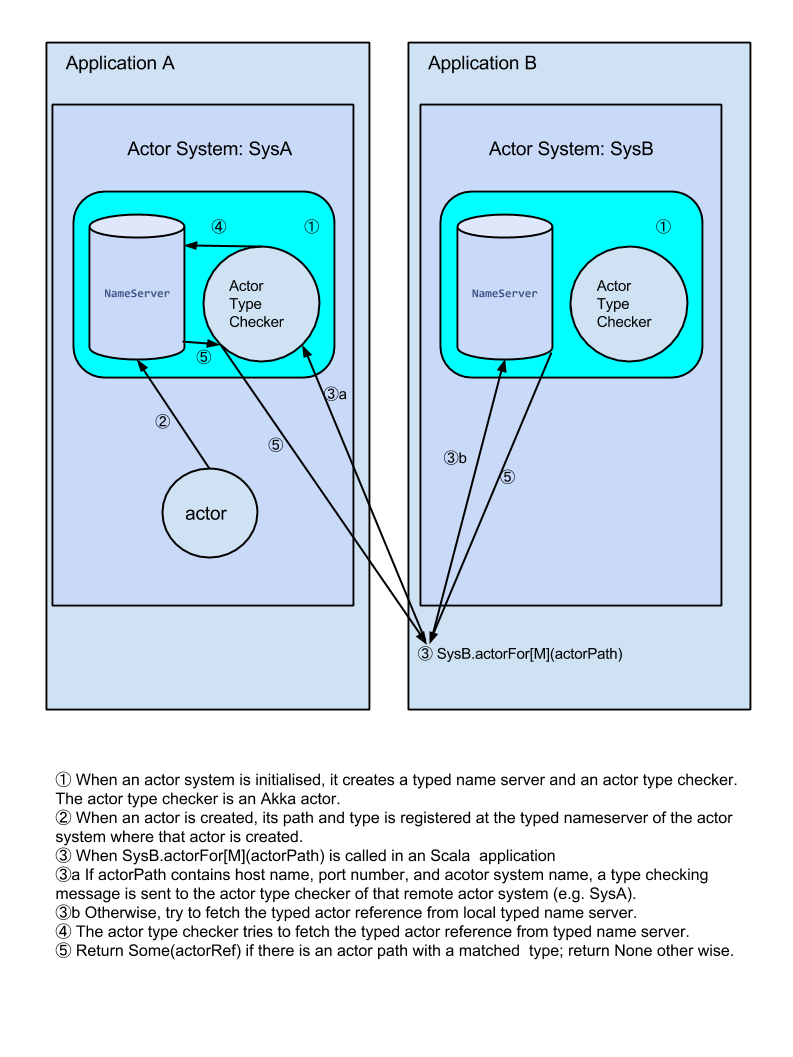
\includegraphics[keepaspectratio=true,height=0.6\paperheight]
{Pictures/RemoteActorReference.png}
    \end{center}
     \caption{Fetched Typed Actor Reference}
   \label{takka_actorFor_fig}
\end{figure}

The {\tt actorOf} method and the {\tt remoteActorOf} method create an actor 
that is supervised by a {\tt user} actor created by the system.  The task of 
creating an actor is delegated to an Akka actor system, which is a private field 
of a TAkka actor system.  The additional work done by the TAkka actor system is 
to register the typed actor path and the typed actor reference into the typed 
name server running in the same JVM (line 17 and line 33 in Figure 
\ref{takka_actorOf} ).  Because an actor reference returned by the Akka  
{\tt actorOf} method cannot be used remotely as it does not contain an IP 
address and a port number, the TAkka library defines a {\tt remoteActorOf} 
method which returns a typed actor reference that contains information 
required for using it remotely.  If remote communication is not enabled by the 
actor system, a {\tt NotRemoteSystemException} will arise.


The {\tt actorFor} method (Figure~\ref{takka_actorFor}) returns a typed actor reference if there is such with 
an expected type located at a given path.  Figure~\ref{takka_actorFor_fig} illustrates how typed name servers 
are used in TAkka to fetch a potentially remote actor reference.  When looking for a typed 
actor reference, the actor system first checks if the input actor path 
contains an IP address and a port number.  If so, it sends a request to the 
{\tt ActorTypeServer} actor in the remote actor system; otherwise it sends a 
request to the {\tt ActorTypeChecker} actor in the local machine.  When an {\tt 
ActorTypeServer} actor receives a request that asks if there is an actor 
reference of the expected type at a given path,
it checks registered names at the typed name server in its JVM.  


Although a typed name server defined in the current TAkka implementation can 
only be directly called by applications running on the same JVM.  As the 
implementation of {\tt actorFor} shows, it can indirectly receive remote 
requests via applications that support distributed communication, for example, 
TAkka actors.  The design of a consistent global shared typed name server is 
left as a future extension.



\section{Supervisor Strategies}
\label{supervision}

The TAkka library uses the Akka supervisor strategies explained in Section 
\ref{akka_supervision}: {\tt OneForOne} and {\tt AllForOne}.  If a supervisor 
adopts the {\tt OneForOne} strategy, it restarts its child when it fails.  
The failure of an actor will not affect its siblings.  If a supervisor adopts 
the {\tt AllForOne} supervisor strategy, all children will 
be restarted when any of them fails.  The third OTP supervisor strategy, {\tt
RestForOne}, restarts children in a user-specified order, and hence is not
supported by Akka as it does not specify an order of initialization for
children.  The {\tt RestForOne} supervisor strategy can be simulated by 
grouping related children and defines special messages to trigger actor 
terminations.  The TAkka library does not implement the {\tt RestForOne} 
strategy because it is not needed for the applications considered in this 
project.

Figure~\ref{takka_supervisor_strategy} gives the API of supervisor strategies in 
TAkka.  In fact, it is the same as the Akka version given in Figure 
\ref{akka_supervisor_strategy}.  TAkka reuses the Akka API because none of the 
supervisor strategies requires type-parameters and TAkka separates 
the message handler for system messages and the message handler for other 
messages.




\begin{figure}[h]
    \begin{lstlisting}    
package akka.actor
abstract class SupervisorStrategy
case class OneForOne(restart:Int, time:Duration)(decider: Throwable => 
  Directive) extends SupervisorStrategy
case class AllForOne(restart:Int, time:Duration)(decider: Throwable => 
  Directive) extends SupervisorStrategy

sealed trait Directive extends AnyRef
object Escalate extends Directive
object Restart extends Directive
object Resume extends Directive
object Stop extends Directive
    \end{lstlisting}
    \caption{TAkka API: Supervisor Strategies}
    \label{takka_supervisor_strategy}
\end{figure}






\begin{comment}
As shown in the API, an Akka supervisor strategy can choose different 
reactions for different reasons of child failures in its {\tt decider} 
parameter.  Recall that {\tt Throwable} is the superclass of {\tt Error} and 
{\tt Exception} in Scala and Java.  Therefore, users can pattern match on 
possible types and values of {\tt Throwable} in the {\tt decider} function.  In 
other words, when the failure of a child is passed to the {\tt decider} 
function of the supervisor, it is matched to a pattern that reacts to that 
failure.

The {\tt decider} function contains user-specified computations and returns a 
value of {\tt Directive} that denotes the standard recovery process implemented 
by the Akka library developers.  The {\tt Directive} trait is an enumerated 
type that has four possible values: the
{\tt Escalate} action which throws the exception to the supervisor of the 
supervisor, the {\tt Restart} action which replaces the failed child with a new 
one, the {\tt Resume} action which asks the child to process the message again, 
and the {\tt Stop} action which terminates the failed actor permanently.


As in OTP, for each supervisor strategy, users can specify the maximum number of
restarts of any child within a period.  The default supervisor strategy in 
TAkka is {\tt OneForOne} that permits unlimited restarts.  {\tt Directive} is 
an enumerated type with the following values: the {\tt Escalate} action which 
throws the exception to the supervisor of the supervisor, the {\tt Restart} 
action which replaces the failed child with a new one, the {\tt Resume} action 
which asks the child to process the message again, and the {\tt Stop} action 
which terminates the failed actor permanently.

\end{comment}

A TAkka Safe Calculator example is given in Figure 
\ref{takka_safe_calculator} as a reminder of the Akka Safe Calculator in 
Figure~\ref{akka_supervised_calculator}. Both examples define a simple 
calculator which supports multiplication and division. The simple calculator 
does not consider the problematic case of dividing a number by 0, in which case 
an {\tt ArithmeticException} will raise. A fault tolerant calculator, safe 
calculator, is defined as the supervisor of the simple calculator. The safe 
calculator delegates calculation tasks to the simple calculator and restarts 
it when an {\tt ArithmeticException} raises. The supervisor 
strategy of the safe calculator also specifies the maximum failures its child 
may have within a time range. If the child fails more frequently than the 
allowed frequency, the safe calculator will be stopped, and its failure will be 
reported to its supervisor, the system guardian actor in this example.  The 
terminal output shows that the simple calculator is restarted before the next 
message is delivered.

The TAkka implementation is modified from the Akka version with changes marked 
in \textcolor{blue}{blue}.  First, an {\tt Operation} trait is introduced as 
the supertype of the {\tt Multiplication} message and the {\tt Division} 
message.  Second, actor classes are parameterized by the type of messages they 
expected.  Third, the {\tt calculator} actor reference in TAkka can publish 
itself as an actor reference, {\tt multiplicator}, which only accepts 
multiplication requests. The supervisor strategy used in the TAkka 
implementation is exactly the same as the one in the Akka implementation.

\begin{figure}[p]
    \begin{lstlisting}[language=scala, escapechar=?]
package sample.takka
import takka.actor.{ActorRef, ActorSystem, Props, Actor}
?\textcolor{blue}{sealed trait Operation}?
case class Multiplication(m:Int, n:Int) ?\textcolor{blue}{extends Operation}?
case class Division(m:Int, n:Int) ?\textcolor{blue}{extends Operation}?
class Calculator extends ?\textcolor{blue}{Actor[Operation]}? {
  def ?\textcolor{blue}{typedReceive}? = {
    case Multiplication(m:Int, n:Int) =>
      println(m +" * "+ n +" = "+ (m*n))    
    case Division(m, n) =>
      println(m +" / "+ n +" = "+ (m/n))
  }
}
class SafeCalculator extends ?\textcolor{blue}{Actor[Operation]}? {
  import language.postfixOps
  override val supervisorStrategy =
    OneForOneStrategy(maxNrOfRetries = 2, withinTimeRange = 1 minute) {
      case _: ArithmeticException  =>
        println("ArithmeticException Raised to: "+self)
        Restart
    }
  val child:ActorRef[Operation] = 
         typedContext.actorOf(Props[Operation, Calculator], "child")
  def ?\textcolor{blue}{typedReceive}? = {    case m => child ! m  }
}
object SupervisorTest extends App{
  val system = ActorSystem("MySystem")
  val calculator:?\textcolor{blue}{ActorRef[Operation]}? = 
        system.actorOf(?\textcolor{blue}{Props[Operation, Calculator]}?, "calculator")
  ?\textcolor{blue}{val multiplicator = calculator.publishAs[Multiplication]}?
  
  calculator ! Multiplication(3, 2)
  multiplicator ! Multiplication(3, 3)
//  multiplicator ! Division(6, 2)  
//  Compiler Error: type mismatch; found : sample.takka.Division 
//  required: 	 sample.takka.Multiplication
  calculator ! Division(10, 0)
  calculator ! Division(10, 5)
}  
/*  Terminal Output:
3 * 2 = 6
3 * 3 = 9
java.lang.ArithmeticException: / by zero
ArithmeticException Raised to: Actor[akka://MySystem/user/safecalculator]
10 / 5 = 2
*/
    \end{lstlisting}
    \caption{TAkka Example: Supervised Calculator}
    \label{takka_safe_calculator}
\end{figure}

\newpage

\section{Fixing The Type Pollution Problem}
\label{type_pollution}

In a system with multiple components, different components may require
different interfaces; since all messages are received in the same
mailbox, a naive approach would be to set the type to the union of all
the interfaces, causing each component to see a type containing
messages not intended for it---an issue dubbed the Type Pollution
Problem.

This section illustrates the Type Pollution Problem and its solution on an
instance of the Model-View-Controller pattern \citep{reenskaug1979original, burbeck87}.  The Model
and View have separate interfaces to the Controller, and neither
should see the interface used by the other.  However, the naive
approach would have the Controller message type contain all the
messages the Controller receives, from both the Model and the View.
A similar problem can occur in a multi-tier architecture \citep{fowler2002patterns},
where an intermediary layer interfaces with both the layer above
and the layer below.

One solution to the type pollution problem is using separate channels
for distinct parties.  For instance, in Model-View-Controller, one
channel would communicate between Model and Controller, and a distinct
channel communicate between Model and View.  Programming models that
support this solution includes the join-calculus \citep{full_join} and
the typed $\pi$-calculus \citep{pi_book}.  Can we gain similar
advantages for a system based on actors rather than channels?

The TAkka solution is to publish a component at different types to different 
parties.  The published type must be a supertype of the most precise type of 
the component.  In Java and Scala applications, this solution can be tricky 
because, as will be briefly discussed in Section~\ref{type_pollution_oo}, a set 
of supertypes must be defined in advance.  
Fortunately, if the component is implemented as a type-parameterized actor, 
the limitation can be avoided straightforwardly.  The demonstration example 
studied in this section is a Tic-Tac-Toe game with a graphical user interface 
(GUI) implemented using the MVC pattern.


\subsection{Case Study: Tic-Tac-Toe}


\subsubsection{The Game}

Tic-Tac-Toe \citep{wiki:tictactoe}, also known as Noughts and Crosses, is a 
paper-and-pencil game.  A basic version of the Tic-Tac-Toe game is played by 
two players who mark X and O in turn in a $3\times3$ grid.  A player wins the 
game if he or she succeeds in placing three respective marks, i.e. three Xs or three Os, in a 
horizontal, vertical, or diagonal row.  The game is drawn if no player wins when 
the grid is fully marked.

Figure~\ref{tictactoe_example} gives an example game won by the first player, 
X.  Figures \ref{fig:t0} to \ref{fig:t7}  are screenshots 
of the game implemented in the next subsection.  The graphical user interface 
of the game contains three parts.  The left hand side of the window shows the 
player with the next move.  The middle of the window shows the current status of 
the game board.  The right hand side contains control buttons, each of which 
kills one component of the application and test if that component will be 
restarted.  Finally, Figure~\ref{fig:t8} announces the winner.

\begin{figure}[p]
     \begin{center}
        \subcaptionbox{ \label{fig:t0}}{
            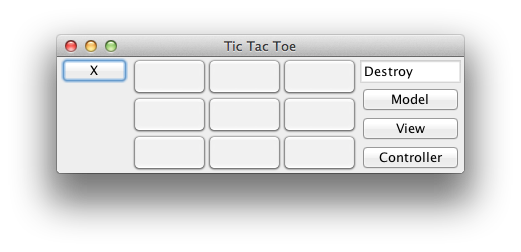
\includegraphics[scale=0.38]{TicTacToeScreenCut/0.png}
        }
        \subcaptionbox{ \label{fig:t1} }{
           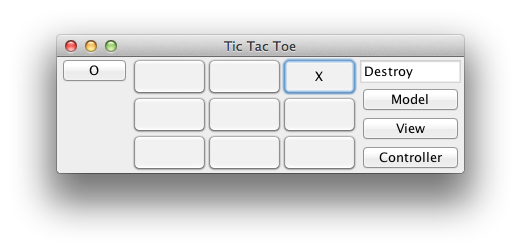
\includegraphics[scale=0.38]{TicTacToeScreenCut/1.png}
        }\\
        \subcaptionbox{ \label{fig:t2} }{
            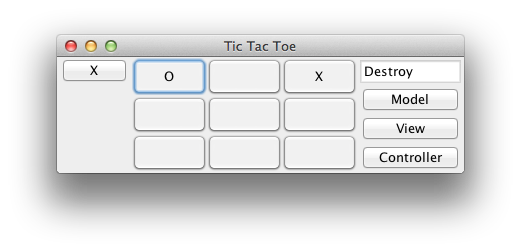
\includegraphics[scale=0.38]{TicTacToeScreenCut/2.png}
        }
        \subcaptionbox{ \label{fig:t3} }{
            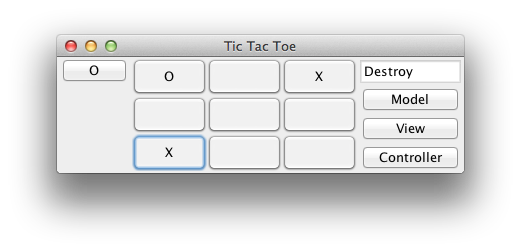
\includegraphics[scale=0.38]{TicTacToeScreenCut/3.png}
        }\\
        \subcaptionbox{ \label{fig:t4} }{
            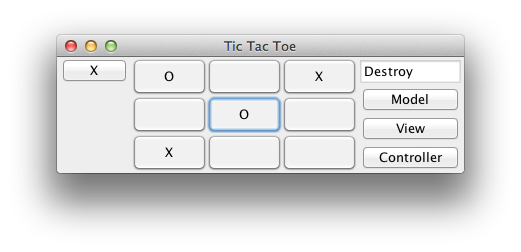
\includegraphics[scale=0.38]{TicTacToeScreenCut/4.png}
        }
        \subcaptionbox{ \label{fig:t5} }{
           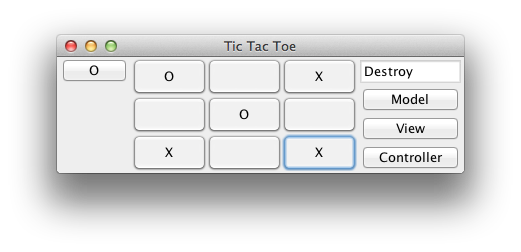
\includegraphics[scale=0.38]{TicTacToeScreenCut/5.png}
        }\\        
        \subcaptionbox{ \label{fig:t6} }{
            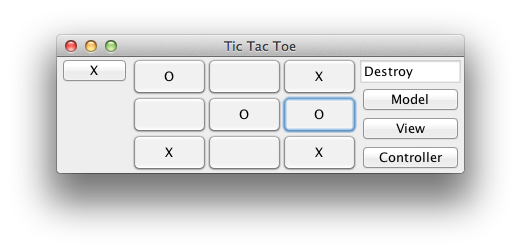
\includegraphics[scale=0.38]{TicTacToeScreenCut/6.png}
        }
        \subcaptionbox{ \label{fig:t7} }{
           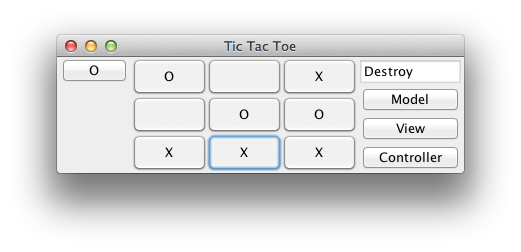
\includegraphics[scale=0.38]{TicTacToeScreenCut/7.png}
        }\\                
        \subcaptionbox{\label{fig:t8}}{
           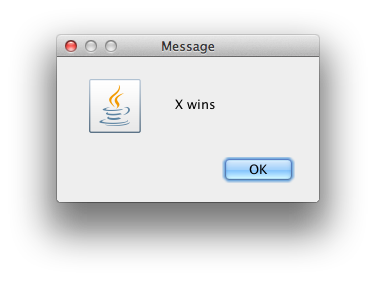
\includegraphics[scale=0.38]{TicTacToeScreenCut/8.png}
        }\\                        
    \end{center}
     \caption{A Game of Tic-Tac-Toe}
   \label{tictactoe_example}
\end{figure}


\subsubsection{The MVC pattern}

Model-view-controller (MVC) is a software architecture pattern introduced by 
\citet{reenskaug1979original}.  The pattern separates the data abstraction
(the model), the representation of data (the view), and the component for 
manipulating the data and interpreting user inputs (the controller).  
In an application built using MVC, a controller coordinates a model and a view, for example,  
sending instructions and reacting to messages from the model and the view.  
Consequently, the controller has two distinct sets of interface: one to
work with the model, the other to work with the view.

MVC has been widely used in the design of applications with a graphical user 
interface (GUI), from early Smalltalk programs written in Xerox Parc 
\citep{reenskaug1979original, reenskaug2003model}, to modern web application 
frameworks like the Zend framework \citep{allen2009zend}, to mobile 
applications including Apple iOS applications \citep{apple:objc}.  This 
section will follow the MVC pattern to implement a Tic-Tac-Toe Game with a 
GUI.  The challenge here is using types to prevent the 
situation where the model sends the controller a message expected from the 
view, or the view pretends to be the model. 
 


\subsection{A TAkka Implementation}




\begin{figure}[p]
\begin{lstlisting}[language=scala, escapechar=?]
package sample.tic_tac_toe.takka

?\textcolor{blue}{sealed trait ControllerMessage}?
?\textcolor{blue}{sealed trait View2ControllerMessage extends ControllerMessage}?
final case class ButtonClickedAt(row:Int, col:Int) extends View2ControllerMessage

?\textcolor{blue}{sealed trait Model2ControllerMessage extends ControllerMessage}?
final case class GridNotEmpty(row:Int, col:Int) extends Model2ControllerMessage
final case class PlayedCross(row:Int, col:Int) extends Model2ControllerMessage
final case class PlayedO(row:Int, col:Int) extends Model2ControllerMessage
final case class NextMove(move:Move) extends Model2ControllerMessage
final case class Winner(move:Move) extends Model2ControllerMessage

?\textcolor{blue}{sealed trait Controller2ViewMessage}?
final case class DisplyError(err:String) extends Controller2ViewMessage
final case class DrawCross(row:Int, col:Int) extends Controller2ViewMessage
final case class DrawO(row:Int, col:Int) extends Controller2ViewMessage
final case class DisplayNextMove(move:Move) extends Controller2ViewMessage
final case class AnnounceWinner(winner:Move) extends Controller2ViewMessage

?\textcolor{blue}{sealed trait Controller2ModelMessage}?
final case class MoveAt(row:Int, col:Int) extends Controller2ModelMessage

final case class ModelSetController(controller:ActorRef[Model2ControllerMessage]) extends Controller2ModelMessage
final case class ViewSetController(controller:ActorRef[View2ControllerMessage]) extends Controller2ViewMessage


sealed trait Move
final case object X extends Move
final case object O extends Move
\end{lstlisting}
\caption{TicTacToe: Message}
\label{TTT_message}
\end{figure}

\begin{figure}[p]

\begin{lstlisting}[language=scala, escapechar=?]
package sample.tic_tac_toe.takka
import takka.actor._
?\textcolor{blue}{final class Model extends Actor[Controller2ModelMessage]}? {
  ?\textcolor{blue}{var controller:ActorRef[Model2ControllerMessage]}? = _  
  def typedReceive = {
    case ModelSetController(control) => controller = control
    case MoveAt(row:Int, col:Int) =>   { model.setStatus(row, col)  }
  }  
  private object model {
    sealed trait GridStatus
    case object Empty extends GridStatus
    case object XModelMove extends GridStatus
    case object OModelMove extends GridStatus // Uppercase O
    
    var nextXMove:Boolean = true // true->X false->O    
    val status:Array[Array[GridStatus]] = 
          Array(Array(Empty, Empty, Empty),
                 Array(Empty, Empty, Empty),
                 Array(Empty, Empty, Empty))
    def setStatus(row:Int, col:Int) = {   
      if(nextXMove){
          if (status(row)(col) == Empty) {
            status(row)(col) = XModelMove
            controller ! PlayedCross(row, col)
            nextXMove = false
            controller ! NextMove(O)
          }else{  controller ! GridNotEmpty(row, col)          }
      }else{
          if (status(row)(col) == Empty) {
            status(row)(col) = OModelMove
            controller ! PlayedO(row, col)
            nextXMove = true
            controller ! NextMove(X)
          }else{  controller ! GridNotEmpty(row, col)          }     
      }

      checkWinner match {
        case Empty =>
        case XModelMove =>          controller ! Winner(X)
        case OModelMove =>          controller ! Winner(O)          
     }}
   def checkWinner:GridStatus = {
     // reuse GridStatus instead of a new set of values
     // return XModelMove if X wins
     // return OModelMove if O wins
     // return Empty if no winner has 
}}
\end{lstlisting}
\caption{TicTacToe: Model}
\label{TTT_model}
\end{figure}

\begin{figure}[p]
\begin{lstlisting}[language=scala, escapechar=?]
package sample.tic_tac_toe.takka

import takka.actor._
import scala.swing._
import scala.swing.event._
import javax.swing.JOptionPane

?\textcolor{blue}{final class View extends Actor[Controller2ViewMessage]}?{
  ?\textcolor{blue}{private var controller:ActorRef[View2ControllerMessage]}? = _
   
  private var guiApp:GUIApplication = _;
      
  def typedReceive = {
     case ViewSetController(control) =>
       assert(controller == null, "controller has been set")
       controller = control
       guiApp = new GUIApplication(controller)
       guiApp.main(Array(""))              
     case DisplyError(err) =>       guiApp.displayError(err)
     case DrawCross(row, col) =>       guiApp.draw(row, col, true)
     case DrawO(row, col) =>       guiApp.draw(row, col, false)
     case DisplayNextMove(move) =>       guiApp.showNextMove(move)
     case AnnounceWinner(winner:Move) => winner match{
       case X => guiApp.announceWinner(true)
       case O => guiApp.announceWinner(false)
     }
  }
}


class GUIApplication(controller:ActorRef[View2ControllerMessage]) extends SimpleSwingApplication {
   def draw(row:Int, col:Int, isCross:Boolean) { 
     // draw X or O at (row, col)
   }
   def showNextMove(move:Move) {
     // update next player
   }
   def displayError(err:String){
     // show error message
   }
   def announceWinner(isCross:Boolean){
     // announce winner
   }
}
\end{lstlisting}
\caption{TicTacToe: View}
\label{TTT_view}
\end{figure}


\begin{figure}[p]
\begin{lstlisting}[language=scala, escapechar=?]
package sample.tik_tak_tok.takka

import takka.actor._

?\textcolor{blue}{final class Controller(model:ActorRef[Controller2ModelMessage], view:ActorRef[Controller2ViewMessage]) extends Actor[ControllerMessage]}? {
  def typedReceive = {
    case ButtonClickedAt(row, col) =>
      model ! MoveAt(row, col)
    case GridNotEmpty(row, col) =>
      view ! DisplyError("grid "+row+" , "+col+" is not empty")
    case PlayedCross(row, col) =>
      view ! DrawCross(row, col)
    case PlayedO(row, col) =>
      view ! DrawO(row:Int, col:Int)
    case NextMove(move) =>
      view ! DisplayNextMove(move)
    case Winner(move) =>
      view ! AnnounceWinner(move)
  }
  
  override def preStart() = {
    model ! ModelSetController(typedSelf.publishAs[Model2ControllerMessage])
    view ! ViewSetController(typedSelf.publishAs[View2ControllerMessage])
  }
}

package sample.tic_tac_toe.takka

import takka.actor._
?\textcolor{blue}{object TicTacToeApplication extends App \{}?
  ?\textcolor{blue}{val system = ActorSystem("LocalTicTacToe")}?
  ?\textcolor{blue}{val model = system.actorOf(Props[Controller2ModelMessage, Model], "model")}?
  ?\textcolor{blue}{val view = system.actorOf(Props[Controller2ViewMessage, View], "view")}?
  ?\textcolor{blue}{val controller = system.actorOf(Props(new Controller(model, view)), "controller")  }?
?\textcolor{blue}{\}}?
\end{lstlisting}
\caption{TicTacToe: Application}
\label{TTT_controller}
\end{figure}

TAkka solves the type pollution problem by using subtyping polymorphism.  The code from 
Figure~\ref{TTT_message} to Figure~\ref{TTT_controller} gives an TAkka 
application that implements the Tic-Tac-Toe game with a GUI.  The code marked 
in \textcolor{blue}{blue} may be reused by other applications built 
using the MVC pattern.


Messages used in this implementation are given in Figure~\ref{TTT_message}. 
Messages sent to the controller are separated into two groups: those expected 
from the model and those expected from the view.  The {\tt Controller} actor of 
this application, defined in Figure~\ref{TTT_controller}, reacts to messages 
sent either from the {\tt Model} actor or the {\tt View} actor.  In its 
initialization process, however, the controller publishes itself as different 
types to the view actor and the model actor.  Although the {\tt publishAs} 
methods in line 22 and line 23 of Figure~\ref{TTT_controller} can be committed 
because the type of the controller has been refined in the {\tt 
ModelSetController} message and the {\tt ViewSetController} message, the code
explicitly expresses the type convention and lets the compiler double check the 
type.

In the definition of the {\tt Model} actor (Figure~\ref{TTT_model}) and the 
{\tt View} actor (Figure~\ref{TTT_view}), the {\tt Controller} actor is declared 
as different types.  As a result, both the view and the model only know the 
communication interface between the controller and itself.  The {\tt Model} 
actor internally represents the game board as a two dimensional array.  Each 
time the model receives a request from the controller, it updates the status of 
the board and then announce the winner or the next player to the controller.  
The {\tt View} actor maintains a GUI application that displays the game board 
and listens to user input.  All user input is forwarded to the controller 
which sends corresponding requests to the model.  When the view receives 
requests from the controller, it updates the game board or announce the winner 
via the GUI.  Detailed GUI implementation is omitted in this thesis for clarity.
Readers can found the complete code in the public code repository of this project. \citep{takka_repo}


Finally, setting up the application is straightforward.  In the code 
given at the bottom of Figure~\ref{TTT_controller}, a {\tt Model} actor, a 
{\tt View} actor, and a {\tt Controller} actor are initialized in a local actor 
system.  In this implementation, the controller actor must be initialized at the 
end because its initialization requires actor references of the model and the 
view.  The user interface of this application looks like the one gives in 
Figure~\ref{tictactoe_example}.  



\subsection{A Scala Interface}
\label{type_pollution_oo}



The type pollution problem is avoided in TAkka by publishing different types of 
an actor to different users.  This method can be applied to any language that 
supports polymorphism.  For example, Figure~\ref{TTT_interface} gives an 
interface of implementing the Tic-Tac-Toe game using the MVC pattern without actors.  The code 
marked in \textcolor{blue}{blue} can be modified for building other 
applications using the MVC pattern.

Similar to the TAkka implementation which separates the type of messages sent 
from a model to a controller and a view to a controller, the interface in Figure 
\ref{TTT_interface} separates the methods of a controller to be called by a 
model and those to be called by a view into two distinct traits.  The controller 
is defined as the subclass of both traits.

The example implementation, however, is difficult to maintain.  Notice that the 
{\tt ControllerForView} trait and the {\tt ControllerForModel} trait are the 
supertypes of the {\tt Controller} trait.  As a result, those two traits 
and their methods should be defined in advance.  Each time a new 
method shall be added to either of the two traits, 
the whole program needs to be recompiled and re-deployed.  Where an application 
is a collaborative project maintained by different groups, attempts at 
large-scale updates should be avoided whenever possible.  

In contrast, our TAkka implementation avoids the problems suffered by the simple
Scala solution because new messages can be added easily as a subtype
of an earlier defined message.   With the benefit of backward compatible behaviour upgrading (Section 
\ref{hot_swapping}), the controller, the model and the view can be updated 
separately.




\begin{figure}[p]
\begin{lstlisting}[language=scala, escapechar=?]
package sample.tic_tac_toe.mvcobject

?\textcolor{blue}{trait Controller extends ControllerForView with ControllerForModel}?
class GameController(model:Model, view:View) extends Controller {
  // implementation
}

?\textcolor{blue}{trait ControllerForView}? {
  def buttonClickedAt(row:Int, col:Int):Unit
}
?\textcolor{blue}{trait ControllerForModel}? {
  def gridNotEmpty(row:Int, col:Int):Unit
  def playedCross(row:Int, col:Int):Unit
  def playedO(row:Int, col:Int):Unit
  def nextMove(move:Move):Unit
  def winner(move:Move):Unit
}

?\textcolor{blue}{trait Model}? {
  ?\textcolor{blue}{def setController(controller:ControllerForModel): Unit}?
  def moveAt(row:Int, col:Int): Unit
}
class GameModel extends Model {
  // implementation
}

?\textcolor{blue}{trait View}? {
  ?\textcolor{blue}{def setController(controller:ControllerForView): Unit}?
  def displyError(err:String): Unit
  def drawCross(row:Int, col:Int): Unit
  def drawO(row:Int, col:Int): Unit
  def displayNextMove(move:Move): Unit
  def announceWinner(winner:Move): Unit
}
class GameView extends View {
  // implementation
}

sealed trait Move
final case object X extends Move
final case object O extends Move

?\textcolor{blue}{object TicTacToeApplication extends App \{}?
  ?\textcolor{blue}{val model = new GameModel;}?
  ?\textcolor{blue}{val view = new GameView;}?
  ?\textcolor{blue}{val controller = new GameController(model, view)  }?
?\textcolor{blue}{\}}?
\end{lstlisting}
\caption{TicTacToe: MVC Interface}
\label{TTT_interface}
\end{figure}


\section{Handling System Messages}
\label{systemmessage}

Actors communicate with each other by sending messages.  To organize actors, a 
special category of messages should be handled by all actors.  In Akka, those 
messages are subclasses of the {\tt PossiblyHarmful} trait.  The TAkka library 
defines messages of the same name as subclasses of the {\tt SystemMessage} trait.


\begin{table}[h]
\begin{center}
\begin{tabular}{| l | c | c | c | c |}
  \hline
  Message & TAkka 2.0 & TAkka 2.1 & Akka 2.0 & Akka 2.1 \\
  \hline
  Kill  & public & public & public & public \\
  \hline
  PoisonPill & public & public & public & public \\
  \hline
  ReceiveTimeout & public & public & public & public \\
  \hline
  ChildTerminated & public & private & public & private \\
  \hline
  Restart & public & private & public & private \\
  \hline
  Terminated & not included & not included & public & public \\
  \hline
  Create  & private & private & public & private \\
  \hline
  Failed  & private & private & public & private \\
  \hline
  Link  & not included & not included & public & private \\
  \hline  
  Unlink  & not included & not included & public & private \\
  \hline 
  Suspend  & private & private & public & private \\
  \hline
  Resume  & private & private & public & private \\
  \hline
\end{tabular}
\end{center}
\caption{System Messages}
\label{system_messages}
\end{table}

Table~\ref{system_messages} lists system messages used in Akka and TAkka.
Some messages are defined as public objects which can be handled by a user where
as some messages are defined as private objects which only be used by the
library developers.  TAkka retains {\tt Kill} and {\tt PoisonPill} because it is used
in the Chaos Monkey library and the Supervision View 
library explained in Section~\ref{reliability}.  TAkka users may also want to use those two messages for
reliability testing.  The {\tt ReceiveTimeout} message is retained because it is used in many 
applications considered in this thesis.  The TAkka library makes {\tt Create}, {\tt Failed}, {\tt Suspend}, 
and {\tt Resume} private because reactions to those messages can be consistently defined
in library rather than leave to users.  The decision is verified by the design
of Akka 2.1, which makes all above messages private as well.  Akka 2.1 also makes
{\tt ChildTerminated} and {\tt Restart} private for the same reason.  The author
does not recognise this point in the design of TAkka 2.0 and follow the Akka design
in TAkka 2.1.  The TAkka library does not retain {\tt Terminated}, {\tt Link}, and {\tt Unlink} because, as will be explained in 
Section~\ref{alternative_designs}, life-cycle monitor relationship outside the 
supervision tree is considered as a redundant design.

The purpose of those messages are examples as the followings.

\paragraph{Kill}   An actor that receives this message will send an {\tt ActorKilledException} 
to its supervisor.

\paragraph{PoisonPill}  An actor that receives this message will be permanently terminated.  The
supervisor cannot restart the killed actor.

\paragraph{ReceiveTimeout}  A message sent from an actor to itself when it has not received a message
after a timeout.

\paragraph{ChildTerminated(child: ActorRef[M])}  A message sent from a child actor to its supervisor before it terminates.
  
\paragraph{Restart}A message sent from a supervisor to its terminated child asking the
child to restart.

\paragraph{Terminated}  When an actor monitors the life cycle of another actor using Akka Death 
Watch \citep[Section 3.1]{akka_doc}, the watcher will receive a 
Terminated(watched) message when the {\it watched} actor is terminated.

\paragraph{Create} A message sent to the created actor itself.
  
\paragraph{Failed}  An actor sends itself a {\tt Failed(cause: Throwable)} message when an error 
of {\tt cause} occurs when it is processing messages.
  
\paragraph{Link} A message sent to linked actors when Akka Death Watch \citep[Section 
3.1]{akka_doc} is used.

\paragraph{Unlink}  A message sent to linked actors when Akka Death Watch \citep[Section 
3.1]{akka_doc} is disabled. 

\paragraph{Suspend}   A message sent by the system to an actor asking it suspend the process of 
processing remaining messages in its mailbox.

\paragraph{Resume}  A message sent by the system to an actor to dissolve the effects of the {\tt 
Suspend} message so that the actor will resume the process of processing 
messages in its mailbox.





The next question is whether a system message should be handled by the library 
or by application developers.  In Erlang and early versions of Akka, all
system messages can be explicitly handled by developers in the {\tt receive}
block.  In recent Akka versions, some system messages become private to library 
developers and some can be still handled by application developers.

As there are only two kinds of supervisor strategies to
consider, both of which have clearly defined operational behaviours, all
messages related to the liveness of actors are handled in the TAkka library. 
Application developers may indirectly affect the system message handler via 
specifying
the supervisor strategies. In contrast, messages related to the behaviour of an
actor, e.g. {\tt ReceiveTimeout}, are better handled by application
developers. In TAkka, {\tt ReceiveTimeout} is the only system message that can
be explicitly handled by users.  Nevertheless, the {\tt SystemMessage}
trait is defined in the library so that new system messages can be included in 
the future when required.

A key design decision in TAkka is to separate handlers for the system messages 
and user-defined messages.  The above decision has two benefits. Firstly,
the type parameter of actor-related classes only need to denote
the type of user defined messages rather than the untagged union of user 
defined messages and the system messages.  Therefore, the TAkka design applies
to systems that do not support untagged union type.  Secondly, since 
system messages can be handled by the default handler, which applies
to most applications, users can focus on the logic of handling user
defined messages.







\section{A Distributed Calculator}
\label{sec_distributed_calculator}

In previous sections, we have seen that an actor can be parameterized by the 
type of messages it expects.  Adding type parameters to actors does not affect 
the construction of supervision trees because system messages are separated 
from other messages.  Because the TAkka library delegates the tasks of actor 
creation and message sending to the underlying Akka system, distributed 
communication can be done in TAkka in the same way as in Akka.  

The example used in this section is modified from the example in \citep[Section 
5.11]{akka_doc}.  In this example, two calculators will be created as actors, 
one basic calculator that can compute addition and subtraction, one 
advanced calculator that can compute multiplication and division.  The basic 
calculator will be created locally as previous examples.  The advanced 
calculator will be created at a remote machine by updating the actor system 
configuration.  Actor references for local and remote actors are retrieved in 
the same way.


\subsection{Actor System Configuration for Distribution}

Application developers can override the default configuration of an Akka actor 
system by providing an alternative {\tt Config} object or load the 
configuration from an {\tt application.conf} file in the application deployment 
folder. \citep{akka_doc}  The configuration of a TAkka actor system is 
modified by changing the {\tt Config} object which is used by the underlying 
Akka actor system.  The details of Akka system configuration are explained in 
the Akka documentation.  This section only explains the configuration used in 
the distributed calculator example.  For details of Akka actor system 
configuration, readers are directed to look at the Akka documentation for the 
version they are using.

The configuration in Figure~\ref{discal_distribute_configuration} is used 
for the {\tt RemoteCreation} system in Figure~\ref{discal_distribute_creation}. 
The configuration overrides three system policies.  Firstly, the system enables 
distributed communication by replacing the actor reference provider from 
{\tt LocalActorRefProvider} to {\tt RemoteActorRefProvider}.  Secondly, the 
{\tt deployment} block specifies that actor created at the logical path  
{\tt /advancedCalculator} shall be physically created by the {\tt 
CalculatorApplication} actor system located at address {\tt 
129.215.91.88:2552}.  Finally, the actor system itself is located at address
{\tt 129.215.91.195:2554}.   In this example, {\tt 129.215.91.88} and {\tt 
129.215.91.195} are two IP addresses allocated for the Ethernet connection at 
the author's office.  {\tt 2552} and {\tt 2554} are port numbers that are not 
used by the two computers used for this test.


\begin{figure}[h]
\begin{lstlisting}
akka{
  actor {
    provider = "akka.remote.RemoteActorRefProvider"
    deployment {
       /advancedCalculator {
         remote = "akka://CalculatorApplication@129.215.91.88:2552"
    }}}
    remote {
       netty {
         hostname = "129.215.91.195"
         port = 2554               
    }
  }
}
\end{lstlisting}
\caption{Configuration Example: Distributed Creation}
\label{discal_distribute_configuration}
\end{figure}

% \newpage
\subsection{A Complete Example}

The classes defined for the example described at the beginning of this section 
are the followings:


\begin{figure}[p]
\begin{lstlisting}
package typed.remote.calculator
import takka.actor.{Actor, ActorRef}
import akka.actor.ActorPath
import scala.reflect.runtime.universe._

trait MathOp
case class Add(nbr1: Int, nbr2: Int) extends MathOp
case class Subtract(nbr1: Int, nbr2: Int) extends MathOp
case class Multiply(nbr1: Int, nbr2: Int) extends MathOp
case class Divide(nbr1: Double, nbr2: Int) extends MathOp

trait CalculatorMessage
case class Op(op:MathOp, sender:ActorRef[MathResult])                    
     extends CalculatorMessage
     
trait MathResult
case class AddResult(nbr: Int, nbr2: Int, result: Int)                   
     extends MathResult
case class SubtractResult(nbr1: Int, nbr2: Int, result: Int)                    
     extends MathResult
case class MultiplicationResult(nbr1: Int, nbr2: Int, result: Int)       
     extends MathResult
case class DivisionResult(nbr1: Double, nbr2: Int, result: Double)       
     extends MathResult
case class Ask(calculator:ActorRef[CalculatorMessage], op:MathOp) 
     extends MathResult
     


class AdvancedCalculatorActor extends Actor[CalculatorMessage] {
  def typedReceive = {
    case Op(Multiply(n1, n2), sender) =>
      println("Calculating %d * %d".format(n1, n2))
      sender ! MultiplicationResult(n1, n2, n1 * n2)
    case Op(Divide(n1, n2), sender) =>
      println("Calculating %.0f / %d".format(n1, n2))
      sender ! DivisionResult(n1, n2, n1 / n2)
  }
}
\end{lstlisting}
\caption{Distributed Calculator: Messages and Advanced Calculator}
\label{discal_message}
\end{figure}

\begin{figure}[p]
\begin{lstlisting}
package typed.remote.calculator
import akka.kernel.Bootable
import takka.actor.{ Props, Actor, ActorSystem }
import com.typesafe.config.ConfigFactory

class SimpleCalculatorActor extends Actor[CalculatorMessage] {
  def typedReceive = {
    case Op(Add(n1, n2), sender) =>
      println("Calculating %d + %d".format(n1, n2))
      sender ! AddResult(n1, n2, n1 + n2)
    case Op(Subtract(n1, n2), sender) =>
      println("Calculating %d - %d".format(n1, n2))
      sender ! SubtractResult(n1, n2, n1 - n2)
  }
}
class CalculatorApplication extends Bootable {
  val system = ActorSystem("CalculatorApplication",
               ConfigFactory.parseString(""" 
                 akka{
                   actor {
                     provider = "akka.remote.RemoteActorRefProvider"
                   }
                   remote {
                     netty {                       
                       hostname = "129.215.91.88"
                       port = 2552       
                     }
                   }
                 }""") )
  val cal = system.actorOf(Props[CalculatorMessage, 
                            SimpleCalculatorActor], "simpleCalculator")
}

object CalcApp {
  def main(args: Array[String]) {
    new CalculatorApplication
    println("Started Calculator Application - waiting for messages")
  }
}
\end{lstlisting}
\caption{Distributed Calculator: Simple Calculator Local Creation}
\label{discal_local_creation}
\end{figure}

\begin{figure}[p]
\begin{lstlisting}
package typed.remote.calculator
import akka.kernel.Bootable
import com.typesafe.config.ConfigFactory
import scala.util.Random
import takka.actor._
class CreationApplication extends Bootable {
  val system = ActorSystem("RemoteCreation", 
                           ConfigFactory.parseString(""" 
                 akka{
                   actor {
                     provider = "akka.remote.RemoteActorRefProvider"
                     deployment {
                       /advancedCalculator {
                         remote = 
                                "akka://CalculatorApplication@129.215.91.88:2552"
                   }}}
                   remote {
                     netty {
                       hostname = "129.215.91.195"
                       port = 2554               
                 }}}""") )
  val localActor = system.actorOf(Props[MathResult, CreationActor],
                                                    "creationActor")
  val remoteActor = system.actorOf(Props[CalculatorMessage, 
                          AdvancedCalculatorActor], "advancedCalculator")
  def doSomething(op: MathOp) = {    localActor ! Ask(remoteActor, op)  }
}
class CreationActor extends Actor[MathResult] {
  def typedReceive = {
    case Ask(calculator, op) => 
      calculator ! Op(op, typedRemoteSelf)      
    case result: MathResult => result match {
      case MultiplicationResult(n1, n2, r) => 
        println("Mul result: %d * %d = %d".format(n1, n2, r))
      case DivisionResult(n1, n2, r)  => 
        println("Div result: %.0f / %d = %.2f".format(n1, n2, r))
}}}
object CreationApp extends App {
    val app = new CreationApplication
    while (true) {
      if (Random.nextInt(100) % 2 == 0) 
         app.doSomething(Multiply(Random.nextInt(20), 
                                      Random.nextInt(20)))
      else app.doSomething(Divide(Random.nextInt(10000),
                                      (Random.nextInt(99) + 1)))
      Thread.sleep(200)
}}

\end{lstlisting}
\caption{Distributed Calculator: Distributed Creation}
\label{discal_distribute_creation}
\end{figure}

\begin{figure}[p]
\begin{lstlisting}
package typed.remote.calculator
import akka.kernel.Bootable
import scala.util.Random
import com.typesafe.config.ConfigFactory
import takka.actor.{ ActorRef, Props, Actor, ActorSystem }

class LookupApplication extends Bootable {
  val system = ActorSystem("LookupApplication", 
                           ConfigFactory.parseString(""" 
                 akka{
                   actor {
                     provider = "akka.remote.RemoteActorRefProvider"
                   }
                   remote {
                     netty {
                       hostname = "129.215.91.195"
                       port = 2553               
                     }
                   }
                 }""") )
  val actor = system.actorOf(Props[MathResult, LookupActor], "lookupActor")
  val remoteActor = system.actorFor[CalculatorMessage]
       ("akka://CalculatorApplication@129.215.91.88:2552/user/simpleCalculator")
  def doSomething(op: MathOp) = {    actor ! Ask(remoteActor, op)  }
}
class LookupActor extends Actor[MathResult] {
  def typedReceive = {
    case Ask(calculator, op) => {      calculator ! Op(op, typedRemoteSelf)    }
    case result: MathResult => result match {
      case AddResult(n1, n2, r)      => 
           println("Add result: %d + %d = %d".format(n1, n2, r))
      case SubtractResult(n1, n2, r) => 
           println("Sub result: %d - %d = %d".format(n1, n2, r))
}}}
object LookupApp extends App {
    val app = new LookupApplication
    while (true) {
      if (Random.nextInt(100) % 2 == 0) 
         app.doSomething(Add(Random.nextInt(100), Random.nextInt(100)))
      else 
           app.doSomething(Subtract(Random.nextInt(100), 
                                        Random.nextInt(100)))
      Thread.sleep(200)
}}

\end{lstlisting}
\caption{Distributed Calculator: Actor Look up}
\label{discal_lookup}
\end{figure}

\paragraph{Operations and Messages} The Operations ({\tt MathOp}) considered in 
this example are addition ({\tt Add}), subtraction ({\tt Subtract}), 
multiplication ({\tt Multiply}), and division ({\tt Divide}).  There are two 
types of messages used in this example: the {\tt CalculatorMessage} sent to a 
real calculator that can computes an operation; the {\tt MathResult} sent to a 
broker who receives calculation requests and display the result of each 
calculation.


\paragraph{Calculators} The two calculator actors defined in this example are 
the \\ {\tt SimpleCalculatorActor} in Figure~\ref{discal_local_creation} and 
the {\tt AdvancedCalculatorActor} in Figure~\ref{discal_message}.  The simple 
calculator can compute addition and subtraction while the advanced calculator 
can compute multiplication and division.


\paragraph{Test Applications} There are three test applications in this example.
The {\tt CalApp} application creates an actor system with name {\tt 
CalculatorApplication} located at address {\tt 129.215.91.88:2552}.  Inside the 
actor system, a simple calculator is created.  The {\tt CreationApp} 
application creates two actors: one {\tt CreationActor} at the local machine 
and one {\tt AdvancedCalculatorActor} at a remote node.  The {\tt 
CreationActor} is used as a broker that sends a request to the advanced 
calculator and print the returned result.  Finally, the {\tt LookupApp} 
application works as the same as the {\tt CreationApp} except that the remote 
actor used in this application is the simple calculator fetched from the 
{\tt actorFor} method.

\vspace{12 pt}

The example code shows that distributed programming is TAkka is enabled in the 
same way as in Akka, that is, by updating the actor system configuration.  For 
an Akka application that enables distributed programming, the same actor system 
configuration can be reused in the corresponding TAkka version.


\section{Design Alternatives}
\label{alternative_designs}

\paragraph{Akka Typed Actor}
In the Akka library, there is a special class called {\tt TypedActor}.
Although an instance of {\tt TypedActor} can be supervised by a
standard actor, it is essentially a different framework as a service
of {\tt TypedActor} class is invoked by a method 
invocation instead of sending a message.  Code in Figure~\ref{akka typed actor} shows 
how to define a simple string processor using Akka typed actor.  
Line 34 to 36 show that a {\tt TypedActor} object does not have a {\tt !} method.
Line 37 to 39 and their output (Line 44 to 45) show that an actor is located at 
the given address but messages sent to that actor using its actor reference are
unhandled.

The Akka {\tt TypedActor} class prevents some type errors but have two limitations. Firstly, {\tt TypedActor} does not 
permit behaviour upgrade.  Secondly, avoiding the type pollution 
problem, explained in Section~\ref{type_pollution}, by 
using Akka typed actors is the same inconvenience as using a simple object-oriented 
model, where supertypes need to be defined in advance.  In Scala and Java, 
introducing a supertype in a type hierarchy requires modification to all 
affected classes, whose source code may not be accessible by application 
developers.


\begin{figure}[p]

\begin{lstlisting}
package sample.akka;

import akka.actor.ActorSystem
import akka.actor.Props
import akka.actor.TypedActor
import akka.actor.TypedProps
import akka.actor.UnhandledMessage

trait StringCounterTypedActor{
  def processString(m:String) 
}

class StringCounterTypedActorImpl (val name:String) extends 
StringCounterTypedActor{
  private var counter = 0;
  def this() = this("default")
  
  def processString(m:String) {
    counter = counter +1
    println("received "+counter+" message(s):\n\t"+m)
  }
}

object StringCounterTypedActorTest extends App {
  val system = ActorSystem("StringCounterTest")
  val counter:StringCounterTypedActor = 
TypedActor(system).typedActorOf(TypedProps[StringCounterTypedActorImpl](), 
"counter")
  counter.processString("Hello World")
  
  val handler = system.actorOf(Props(new MessageHandler()))
  system.eventStream.subscribe(handler,classOf[akka.actor.UnhandledMessage]);
  
//  counter ! "Hello World"  
//  Compiler Error:  
//   value ! is not a member of sample.akka.StringCounterTypedActor
  val counterRef = system.actorFor("akka://StringCounterTest/user/counter")
  counterRef ! "Hello World Again"
  counterRef ! 2
}
/*  Terminal Output:
received 1 message(s):
	Hello World
unhandled message:Hello World Again
unhandled message:2
 */		
\end{lstlisting}
\caption{Akka Example: String Counter using Akka TypedActor}
\label{akka typed actor}
\end{figure}



\paragraph{Actors with or without Internal Mutable States}
The actor model formalized by \citet{Hewitt:1973} does not 
specify its implementation strategy.  In Erlang, a functional programming 
language, actors do not have mutable states.  It is recommended that the state 
of an actor, if there is any, to be saved in an {\it ETS} table, a data structure 
provided by the OTP library \citep{ErlangManual}.  In Scala, users are free
to use mutable variables in code.
The TAkka library is built on top of Akka and implemented in Scala.  
As a result, TAkka does not prevent users from defining actors with 
mutable states.  
Nevertheless, the author of this thesis encourages the use of 
actors in a functional style, for example encoding the {\tt sender} of a 
synchronous message as part of the incoming message rather than a state 
of an actor, because it is difficult to synchronize mutable
states of replicated actors in a cluster environment.

In a cluster, resources are replicated at different locations to provide 
fault-tolerant services.  The CAP theorem \citep{CAP} states that it is
impossible to achieve consistency, availability, and partition tolerance in a
distributed system simultaneously.  For actors that use mutable state, system 
providers have to either sacrifice 
availability or partition tolerance, or modify the consistency model.  For 
example, Akka actors have mutable state and Akka cluster developers
expand a great deal of effort to implement an eventual consistency model \citep{Kuhn12}.
In contrast, stateless services, e.g. RESTful web services 
\citep{Fielding:2002}, are more likely to achieve a good scalability and 
availability.



\paragraph{Bi-linked Actors}
In addition to one-way linking in the supervision tree, Erlang and Akka
provide a mechanism to define two-way linkage between actors. 
Bi-linked actors are aware of the liveness of each other.  The author believes 
that bi-linked actors are redundant in a system where supervision is
obligatory.  Notice that, if the computation of an actor relies on the liveness
of another actor, those two actors should be organized in the same 
supervision tree.

\section{Summing Up}

This chapter presents the design and implementation of the TAkka library.
In TAkka, an actor reference is parameterized by the type of the messages 
expected by the actor.  Similarly type parameter is added to the {\tt Actor} 
class, the {\tt Prop} class and the {\tt ActorContext} class.  The TAkka 
library uses both static and dynamic type checking so that type errors are 
detected at the earliest opportunity.  To enable look up on remote actor 
references, TAkka defines a typed name server that keeps maps from typed 
symbols to values of the corresponding types.    

The TAkka library adds type checking features to the Akka library but delegates 
tasks such as actor creation and message passing to the underlying Akka 
systems.  This chapter shows that, by separating the handler for system 
messages and other messages, supervision tree and remote 
communication can be done in the same way as in the Akka library. 


